\chapter{LND instrument}
\label{chp:GCS_Python}

\section{temperature variation of the LND instrument from 2019 to 2023}

Inside of the sensor head, LND has several temperature measusment sensor, monitoring the temperature variation of the chips and the surrounding temperature, as shown in Fig.\ref{}. The temperature sensor only operates together with LND on the day time. 
The temperature variation on the lunar surface

\begin{figure}
    \centerfloat
    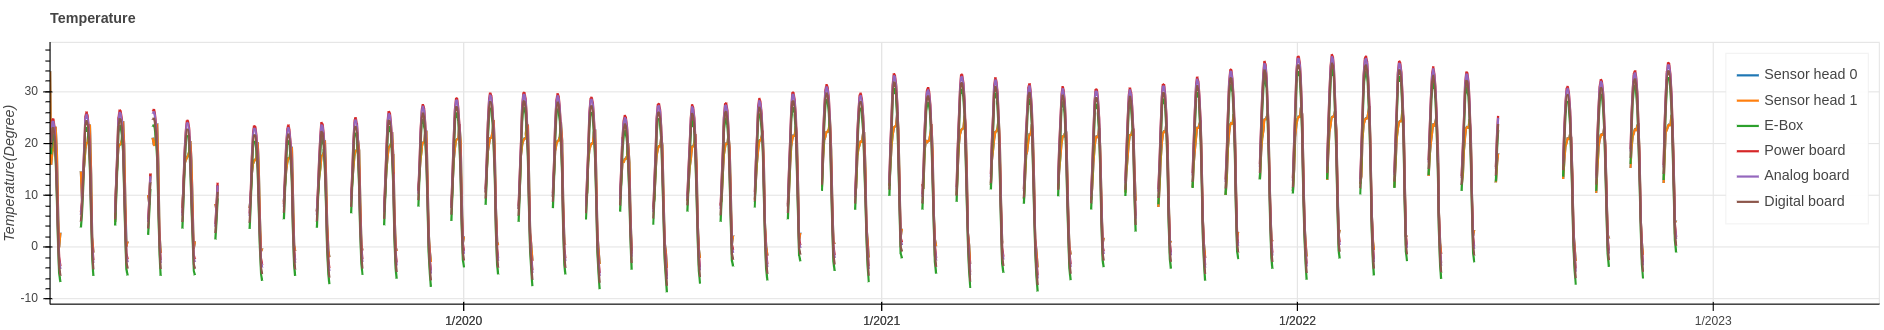
\includegraphics[angle = 90, width = \textwidth, height = \textheight]{images/lnd_temperature.png}
    \caption{LND temperature variations}
    \label{}
\end{figure}


\section{The overall proton, helium and TID variation and the most updated SEP list}

\begin{figure}
    \centerfloat
    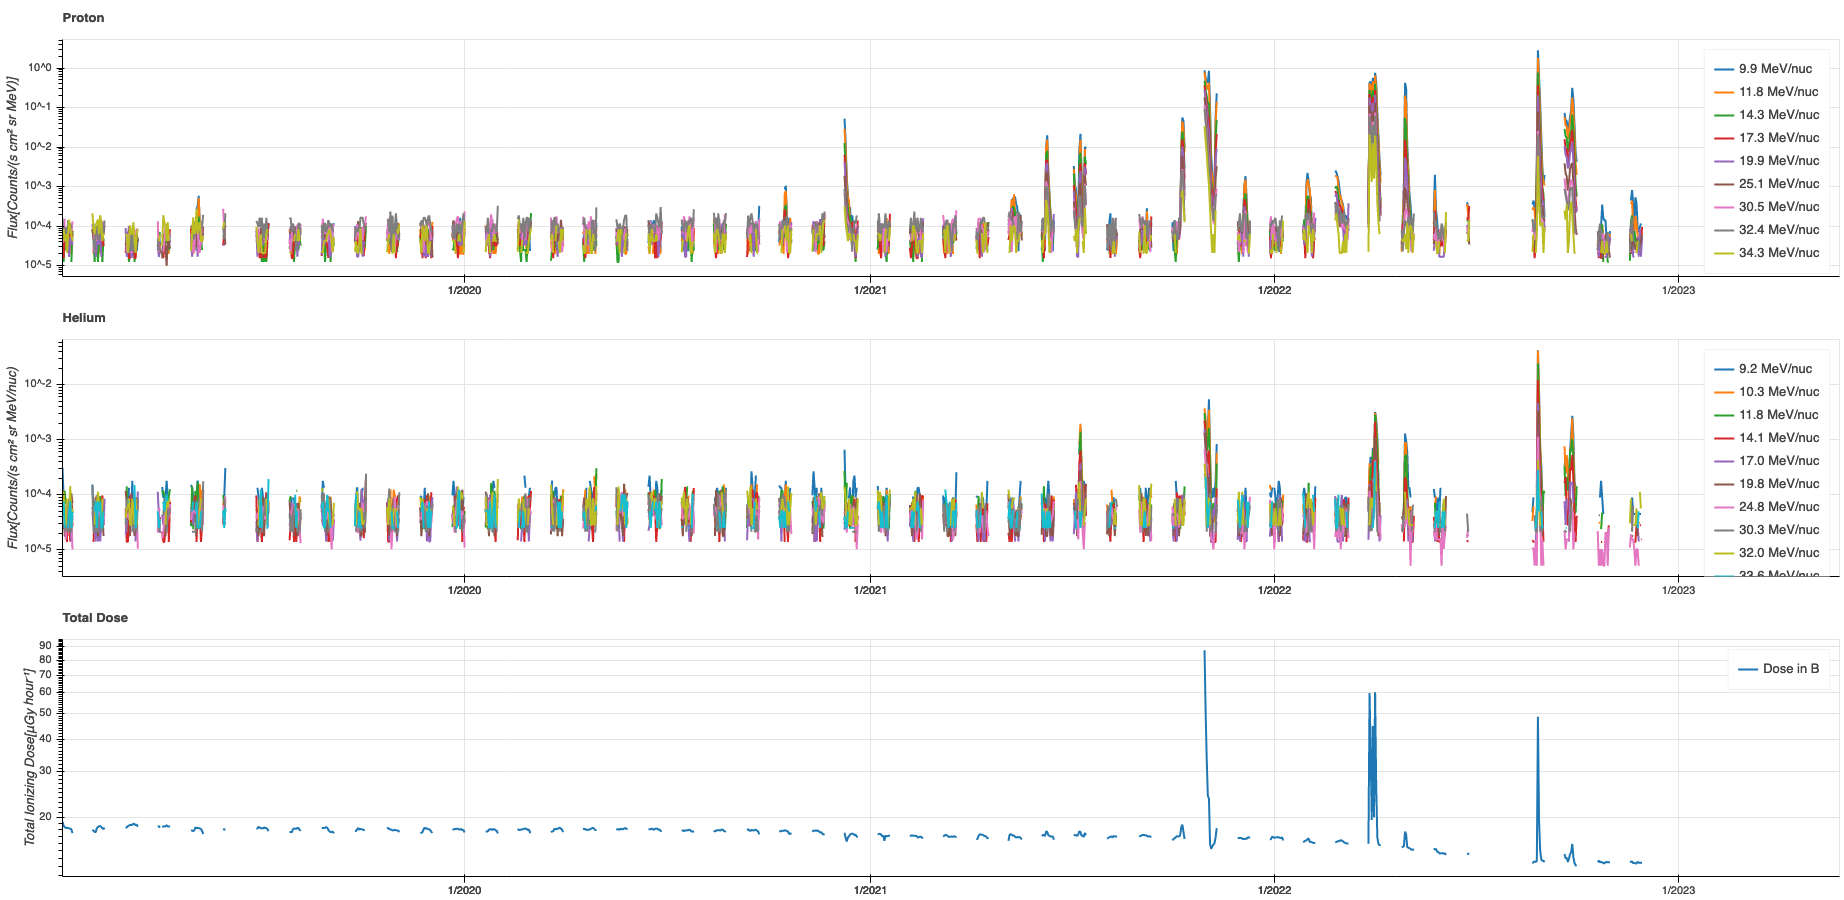
\includegraphics[angle = 90, width = 0.9\textheight, height = 0.8\textwidth]{images/LND-proton-helium-TID.png}
    \caption[The overview variation of proton and helium flux and \ac{TID}]{The proton, helium flux and hourly averaged \ac{TID} temporal variation from 2019 to 2023, based on the measurement from \ac{LND} on the lunar surface}
    \label{Fig:appendix_LND_proton_helium_TID}
\end{figure}

The above figures are generated by the LND webplotter which is a web application that is used to visualize the LND measurement in a quick and fast way. 
Currently, the webplotter is running in a server named etsasa located in the IEAP.
The webplotter is written in Python and the source code is available in the github repository \url{https://gitlab.physik.uni-kiel.de/LND/lnd_webplotter}. 
Inner used webplotter 
Created by Zigong Xu. following the tempelate of SOLO loader

2021 August, Lid problem. Beside, malfunction of the LND lid.

% create a table of SEP list that LND measured
\begin{table}[!h]
    \centering
    \caption[The SEP event list observed on LND]{The SEP event list observed on LND between 2019 and 2022}
\begin{tabular}{cccccc}
    \hline
    No.     & Lunar day & Start time    & End time      & Radiation hazard  & Peak energy\\
    \hline
    1       & 1         &               &               &  &\\
    2       & 1         &               &               &   &\\
    3       & 1         &               &               &   &\\
    4       & 1         &               &               &   &\\    
    \hline
\end{tabular}
\label{Tab:appendix_LND_SEP_list}
\end{table}

\section{Correction of the LND bias current and voltage}

\begin{figure}
    \centerfloat
    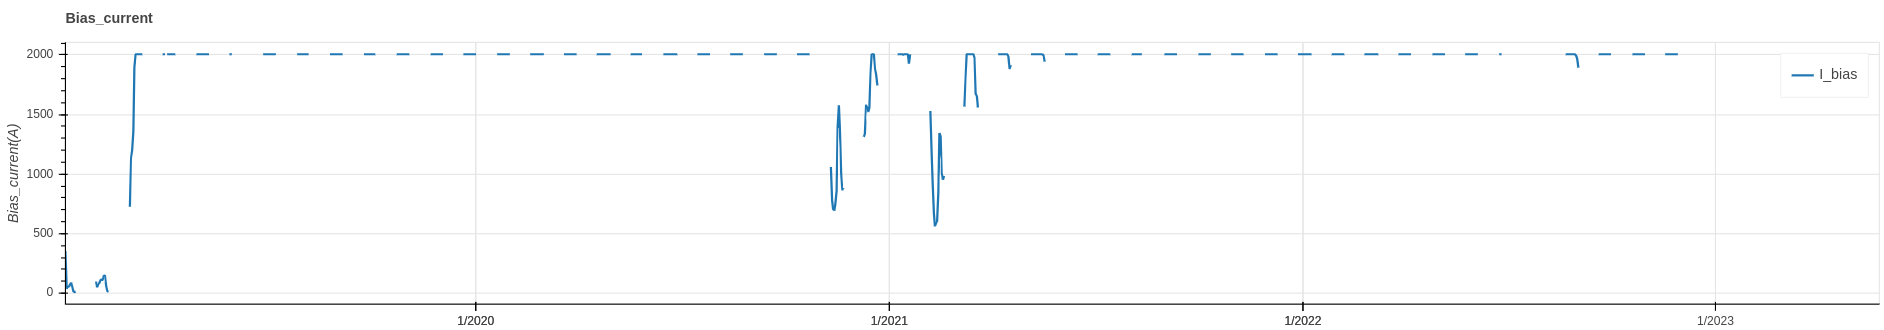
\includegraphics[angle = 90]{images/lnd_bias_current.png}
    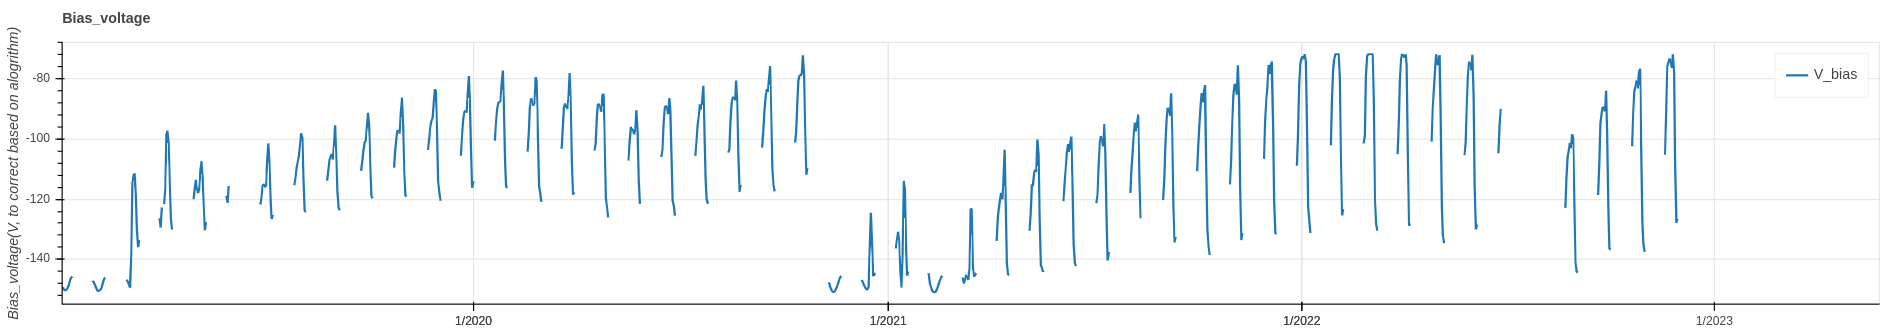
\includegraphics{images/lnd_bias_voltage.png}
    \caption{}
    \label{}
\end{figure}


    Due to the noise of the detectors, the bias current reach the limit of the meaurements at 2$\mu$A. 

Below are the scripts used to calculate the correct bias voltage and current that measured on the LND instrument from Stephan B¨ottcher (private communication), who is the desinger of the LND instruement hardware and software in the IEAP.
\begin{lstlisting}[language=Python]
function Ibias() {
    a = $(HK_Ibias+3)
    if (a>4000) a = (147.3 + degC($(HK_T_LVPS+3))*0.164 - $(HK_Vbias+3)*0.05488) / 0.01810
    return a*0.4928
}

function Vbias() {
    return $(HK_Vbias+3)*0.05488 + $(HK_Ibias+3)*0.01810
}

\end{lstlisting}

\section{Discrepanchy between LND and CREME}

\section{Heavy ion spectra}

\section{He3 spectra}
Mostly the instrument effect, the He3 spectra is not reliable.

\section{L1 responce simulation}

